\documentclass[12pt,a4paper]{article}
\usepackage[utf8]{inputenc}
\usepackage[portuguese]{babel}
\usepackage[T1]{fontenc}
\usepackage{amsmath}
\usepackage{amsfonts}
\usepackage{amssymb}
\usepackage{graphicx}
\usepackage{times}
\usepackage{wrapfig}
\usepackage{calligra}
\usepackage{indentfirst}
\usepackage{hyperref}
\usepackage{xcolor}
\usepackage{tikz}
\usepackage{pgfplots}
\pgfplotsset{compat=1.15}
\usepackage{mathrsfs}
\usetikzlibrary{arrows}
\usepackage[left=2cm,right=2cm,top=2cm,bottom=2cm]{geometry}
\usepackage{multicol}
\author{Eduardo Adame}
\title{Pacotes}

\hypersetup{
    colorlinks=true,
    linkcolor=blue,
    filecolor=magenta,      
    urlcolor=green,
}
\definecolor{airforceblue}{rgb}{0.36, 0.54, 0.66}
\definecolor{uuuuuu}{rgb}{0.26666666666666666,0.26666666666666666,0.26666666666666666}
\definecolor{zzttqq}{rgb}{0.6,0.2,0}
\definecolor{xdxdff}{rgb}{0.49019607843137253,0.49019607843137253,1}
\begin{document}

\maketitle
\newpage
\tableofcontents
\newpage

\section{Texto em Latim}
Lorem ipsum dolor sit amet, consectetur adipiscing elit. Praesent at aliquam tellus. Suspendisse ut pulvinar ante. Suspendisse mi nisi, tincidunt at nisi id, commodo porta nisl. Curabitur in varius velit, non dignissim urna. Maecenas consectetur urna quis mi tincidunt, at convallis nibh porttitor. Nullam a ultricies massa. Sed eleifend scelerisque sollicitudin. Nunc varius vulputate purus at viverra. Duis ligula tellus, ultrices nec ex eu, rhoncus tempor augue. Vivamus dignissim nisl nisl, a egestas mi mollis congue. Praesent orci est, egestas tempor odio at, iaculis rutrum ipsum. Etiam sollicitudin tempor mauris, tincidunt rhoncus justo fermentum sed.
\section{Texto em Multi-Colunas}
\begin{multicols}{2}
Donec finibus massa et odio facilisis, sed sodales ligula scelerisque. Vivamus vehicula cursus volutpat. Aliquam sit amet diam venenatis, tincidunt diam eu, ultrices enim. Nunc ornare nulla nec molestie tincidunt. Curabitur magna diam, interdum id felis vel, blandit suscipit erat. Aenean orci ante, pulvinar non lacus ut, dapibus efficitur elit. Aliquam blandit sodales metus ut facilisis. Mauris sit amet sapien eu dolor feugiat mollis. Proin in risus fringilla nisl dignissim ornare vel sed metus. Vestibulum felis magna, commodo ullamcorper arcu ut, auctor hendrerit augue. Phasellus sit amet gravida ligula. Integer tempus massa in blandit luctus. Integer luctus lectus libero, in viverra justo aliquam quis. Praesent leo nibh, fringilla vitae bibendum in, pellentesque eu odio. Duis urna mi, lobortis sed tellus a, mollis bibendum eros. Aliquam consequat, felis sit amet euismod viverra, tellus odio congue nibh, volutpat convallis augue augue vel metus.
\end{multicols}
\section{Figura no Meio do Texto}
\begin{wrapfigure}{R}{.3\textwidth}
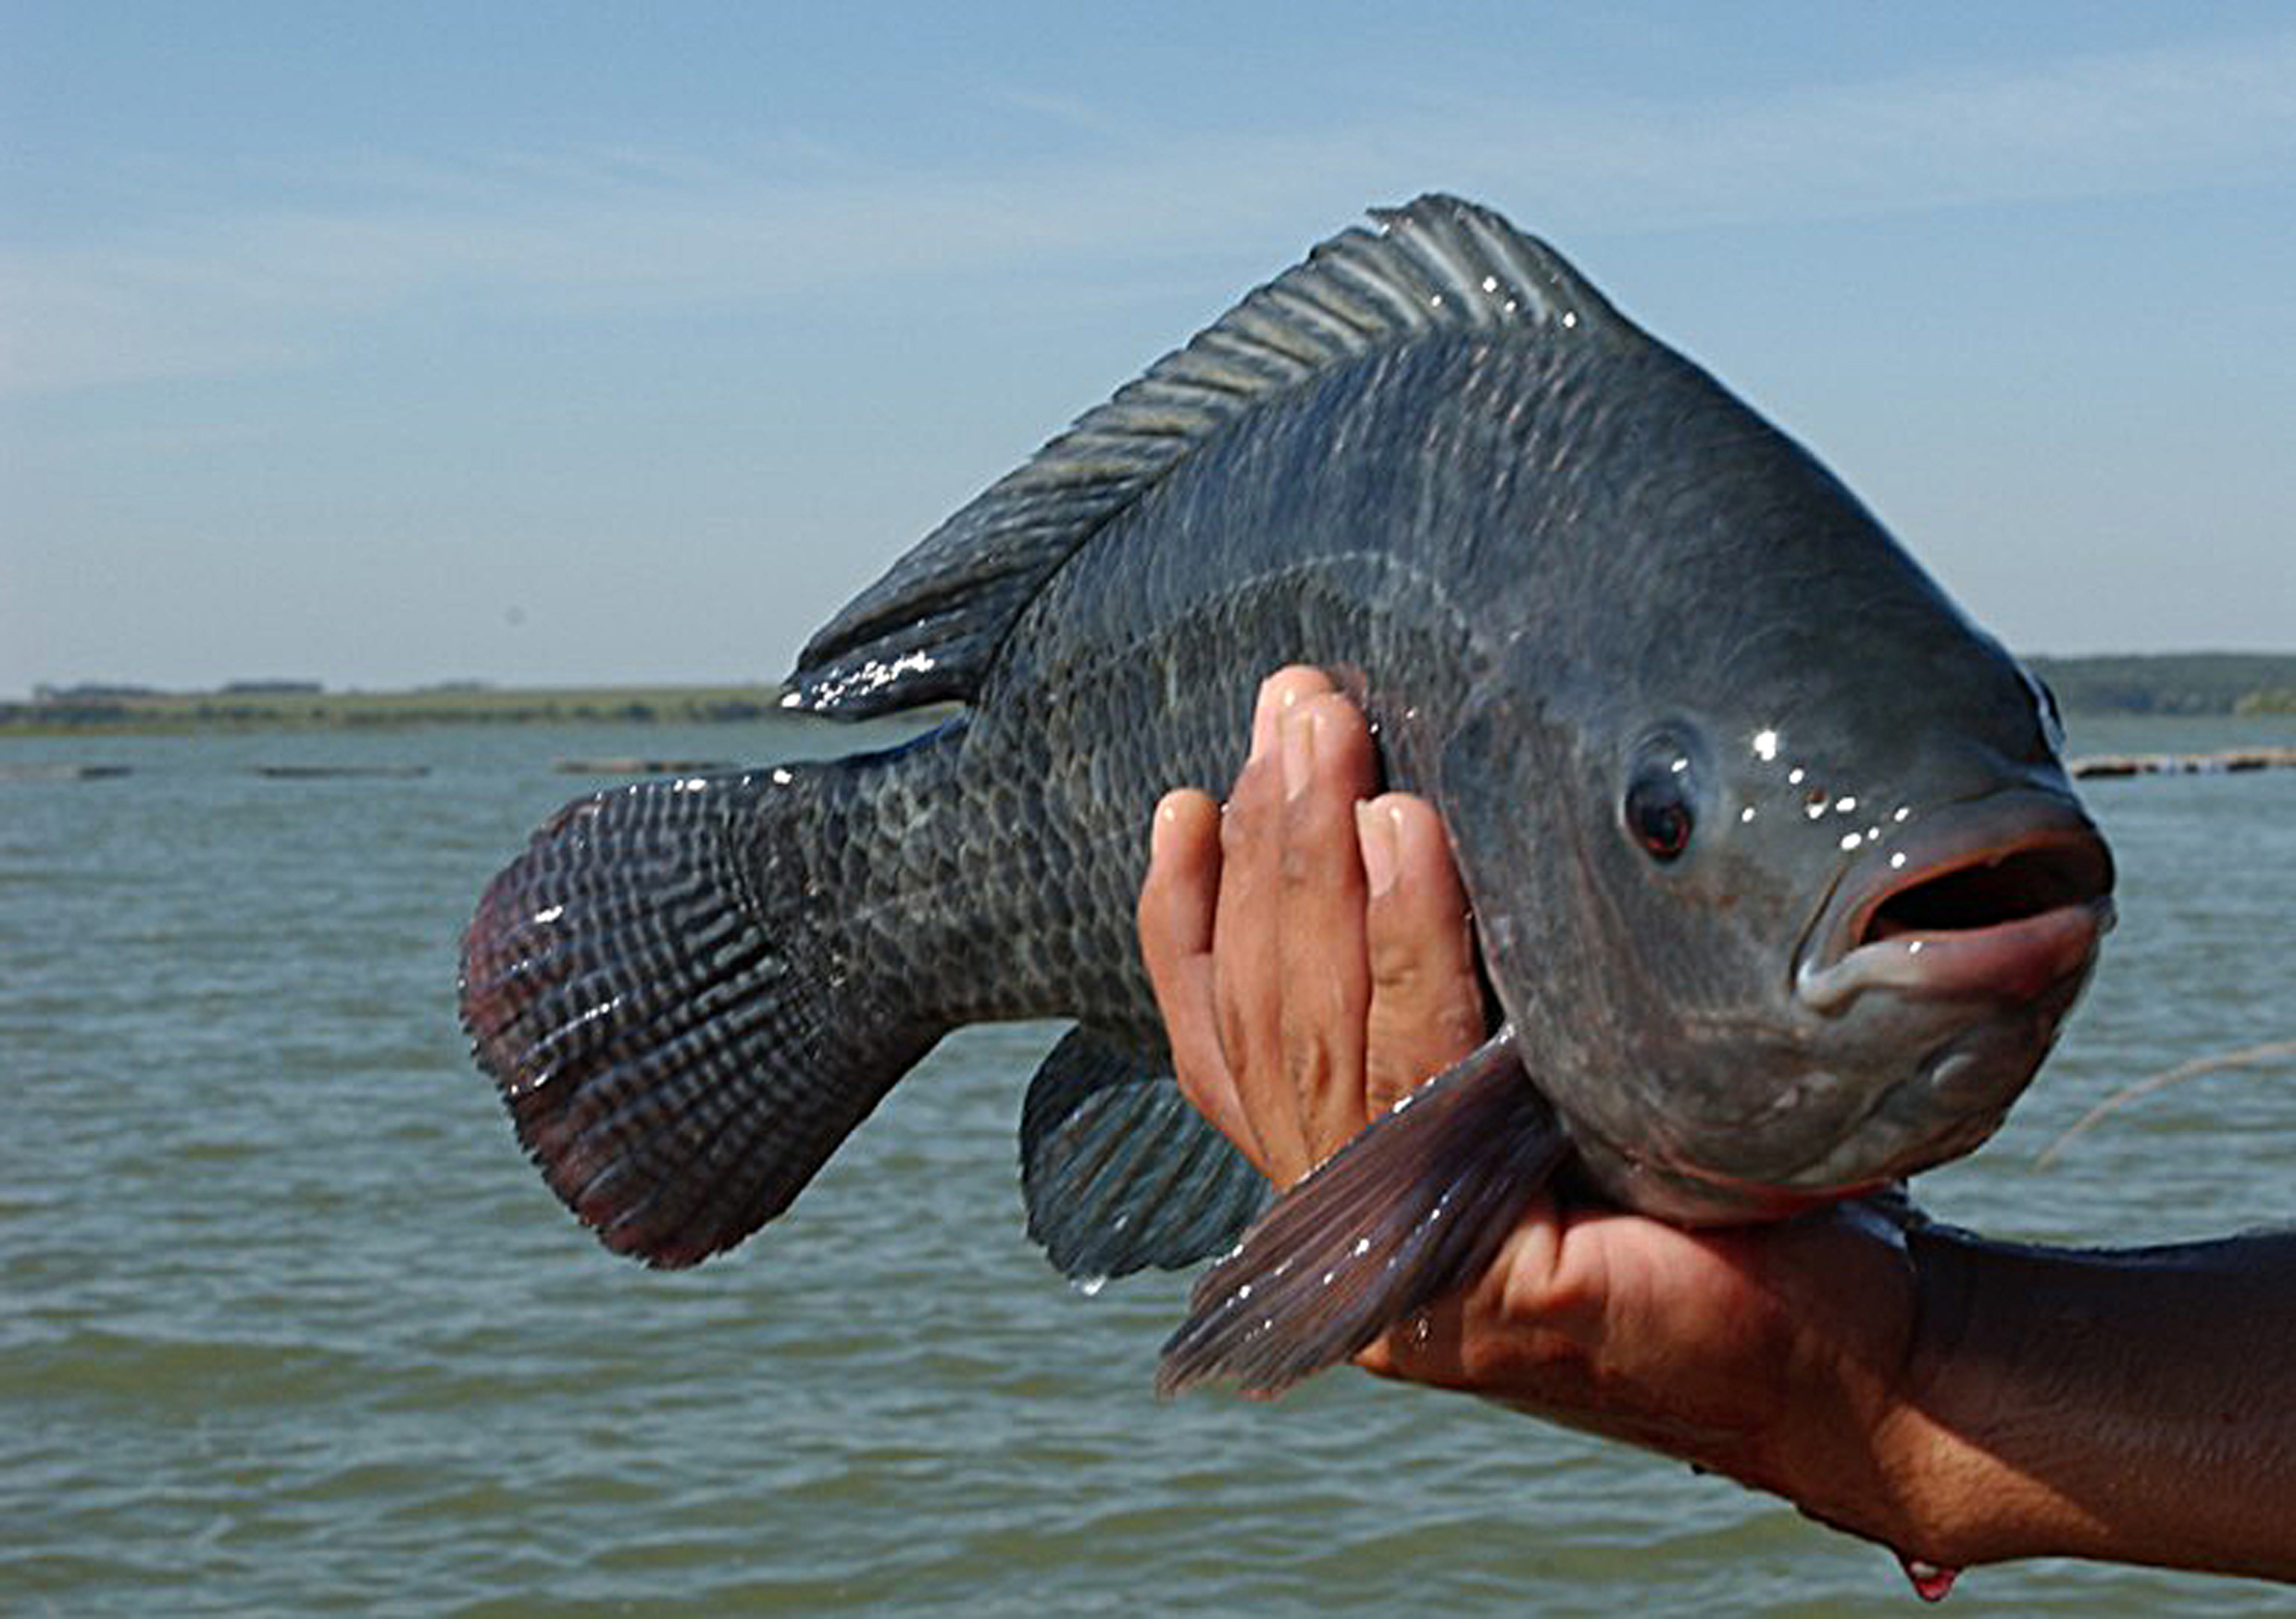
\includegraphics[width=.3\textwidth]{peixe.jpg}
\caption{Peixe Bacana}
\end{wrapfigure}
Donec consectetur ut lectus ut porta. Curabitur a ante accumsan, ullamcorper nunc id, accumsan nibh. Maecenas consequat, arcu ultricies volutpat finibus, justo eros efficitur nulla, ac semper lacus elit a neque. Nam et orci nisi. Suspendisse eget nulla ultricies, condimentum nisi vitae, pharetra ante. Pellentesque habitant morbi tristique senectus et netus et malesuada fames ac turpis egestas.
Suspendisse ut orci eget odio pulvinar eleifend. Proin in sapien mattis, pharetra sapien id, porta quam. Mauris a sapien lobortis, lobortis tellus elementum, finibus ex. Aliquam ac est ex. Etiam quis placerat nunc, ut mollis sem. Phasellus ac sem mattis, imperdiet erat et, lobortis neque. Class aptent taciti sociosqu ad litora torquent per conubia nostra, per inceptos himenaeos. Integer ultrices, diam quis bibendum mattis, leo sem lacinia augue, vitae fermentum est ligula quis lorem.\footnote{Latim}

\begin{figure}[!b]
{\calligra Eduardo Adame Salles}
\end{figure}
\href{https://github.com/adamesalles}{LINK PARA O MEU GITHUB}

\newpage
\section{Texto Colorido}
\textcolor{red}{R: 100 kN} 

\textcolor{yellow!70!cyan}{Look at the stars} 

\textcolor{airforceblue}{TEXTO TESTE}

\section{Ilustrações}
Veja a ilustração abaixo:
\begin{figure}[!h]
\centering
\begin{tikzpicture}
\draw[->, blue] (0,0) -- (1,2);
\draw[fill = blue!40] (2,0) -- (3,0) -- (3,1) -- (2,1) -- cycle;
\end{tikzpicture}
\end{figure}

\begin{tikzpicture}[line cap=round,line join=round,>=triangle 45,x=1cm,y=1cm]
\begin{axis}[
x=1cm,y=1cm,
axis lines=middle,
ymajorgrids=true,
xmajorgrids=true,
xmin=-7.751705484598046,
xmax=6.944012021036821,
ymin=-2.523200601051839,
ymax=6.222103681442521,
xtick={-7,-6,...,6},
ytick={-2,-1,...,6},]
\clip(-7.751705484598046,-2.523200601051839) rectangle (6.944012021036821,6.222103681442521);
\fill[line width=2pt,color=zzttqq,fill=zzttqq,fill opacity=0.10000000149011612] (-2,0) -- (0,2) -- (-2,4) -- (-4,2) -- cycle;
\draw [line width=2pt,color=zzttqq] (-2,0)-- (0,2);
\draw [line width=2pt,color=zzttqq] (0,2)-- (-2,4);
\draw [line width=2pt,color=zzttqq] (-2,4)-- (-4,2);
\draw [line width=2pt,color=zzttqq] (-4,2)-- (-2,0);
\begin{scriptsize}
\draw [fill=xdxdff] (-2,0) circle (2.5pt);
\draw[color=xdxdff] (-1.8764237415477056,0.32428249436513906) node {$A$};
\draw [fill=xdxdff] (0,2) circle (2.5pt);
\draw[color=xdxdff] (0.12207362885049218,2.3227798647633344) node {$B$};
\draw[color=zzttqq] (-2.1168444778362105,2.1424643125469562) node {$Quadrado$};
\draw [fill=uuuuuu] (-2,4) circle (2.5pt);
\draw[color=uuuuuu] (-1.8764237415477056,4.3212772351615305) node {$C$};
\draw [fill=uuuuuu] (-4,2) circle (2.5pt);
\draw[color=uuuuuu] (-3.8749211119459037,2.3227798647633344) node {$D$};
\end{scriptsize}
\end{axis}
\end{tikzpicture}
\end{document}